\documentclass[12pt]{article} % Default font size is 12pt, it can be changed here

\usepackage{siunitx}
%\usepackage{apacite}
\usepackage{amsmath}
\usepackage[utf8]{inputenc}
\usepackage{geometry} % Required to change the page size to A4
\geometry{a4paper} % Set the page size to be A4 as opposed to the default US Letter
\setlength{\parindent}{4em}
\usepackage{graphicx} % Required for including pictures
\usepackage[portuguese]{babel}
\usepackage{indentfirst}
\usepackage{float} % Allows putting an [H] in \begin{figure} to specify the exact location of the figure
\usepackage{wrapfig} % Allows in-line images such as the example fish picture
\usepackage{setspace}
\usepackage{courier}
\usepackage{caption}
\usepackage{subcaption}
\usepackage{lipsum} % Used for inserting dummy 'Lorem ipsum' text into the template
\usepackage{blindtext}
\usepackage{scrextend}
\usepackage{enumitem}
\usepackage{listings}
\usepackage{xcolor}
\usepackage{eurosym}
\usepackage{titlesec}

\titleformat{\paragraph}
{\normalfont\normalsize\bfseries}{\theparagraph}{1em}{}
\titlespacing*{\paragraph}
{0pt}{3.25ex plus 1ex minus .2ex}{1.5ex plus .2ex}



\linespread{1.2} % Line spacing

\graphicspath{{./Pictures/}}
%%%/////////////////////////////TITLE//////////////////////////////////////////%%
\begin{document}
	\begin{titlepage}
	\newcommand{\HRule}{\rule{\linewidth}{0.5mm}} % Defines a new command for the horizontal lines, change thickness here
	\center % Center everything on the page
	\textsc{\LARGE Universidade do Minho}\\[1.5cm] % Name of your university/college

	\begin{figure}[!htbp]
		
\includegraphics[width=5cm]{ola.png}
		\centering
	\end{figure}

	\textsc{\Large Mestrado Integrado em Engenharia de Telecomunicações e Informática}\\[1cm] % Major heading such as course name
	\textsc{\large Projeto de Telecomunicações e Informática I}\\[0.5cm] % Minor heading such as course title
	
	\HRule \\[0.4cm]
	{ \huge \bfseries Relatório Fase A}\\[0.4cm] % Title of your document
	\HRule \\[1cm]

		\begin{minipage}{0.4\textwidth}
			\begin{flushleft} \large
				\emph{Autores:}\\
				Gilberto Morim, A65214\\
				João Costa, A76451\\
				Tiago Teles, A76266\\ % Your name
			\end{flushleft}
		\end{minipage}
~
		\begin{minipage}{0.4\textwidth}
			\begin{flushright} \large
				\emph{Docentes:} \\
				António Costa \\
				Helena Rodrigues % Supervisor's Name
			\end{flushright}
		\end{minipage}\\[2cm]

	{\large \today}\\[3cm] % Date, change the \today to a set date if you want to be precise

		\vfill % Fill the rest of the page with whitespace
\end{titlepage}
\tableofcontents
\newpage

%INTRODUÇÃO
\section{Introdução}
No âmbito da unidade curricular de Projeto de Telecomunicações e Informática I, foi solicitado aos alunos o desenvolvimento de um projeto que consiste num sistema de \textit{software} que disponibiliza um serviço de posicionamento de utilizadores num dado espaço. Este serviço é baseado em Wi-Fi \textit{fingerprint} e em \textit{crowdsourcing}. Em adição, uma aplicação será desenvolvida na qual informa aos utilizadores as suas respetivas posições dentro de um espaço como também as posições vizinhas.\par

Para a presente fase deste projeto, pretendemos fazer uma apresentação de todo o planeamento que visamos ter para este projeto. Serão expostas as ideias e funcionalidades que concluímos (numa visão inicial) para o sistema de serviço de posicionamento.\par
\text{}\par
Os tópicos de maior relevância a serem apresentados são:

\begin{center}
	\begin{minipage}{3.0\linewidth}
		\begin{itemize}
			\item Arquitetura do sitema;
			\item Componentes da infraestrutura de \textit{software} e aplicações;
			\item Modelos de dados;
		\end{itemize}
	 \end{minipage}
\end{center}

\pagebreak

\section{Arquitetura do sistema}
A arquitetura do sistema permite-nos ter uma perspetiva geral de como o serviço de posicionamento será constituído e que interações existem entre cada componente a implementar. A figura abaixo, Figura 1, representa a arquiteura geral do sistema de posicionamento e é composta por três elementos: Um servidor \textit{Web}, uma aplicação gestora e uma aplicação móvel. Cada componente será explicada no tópico a seguir.\par

\begin{figure}[!htbp]
		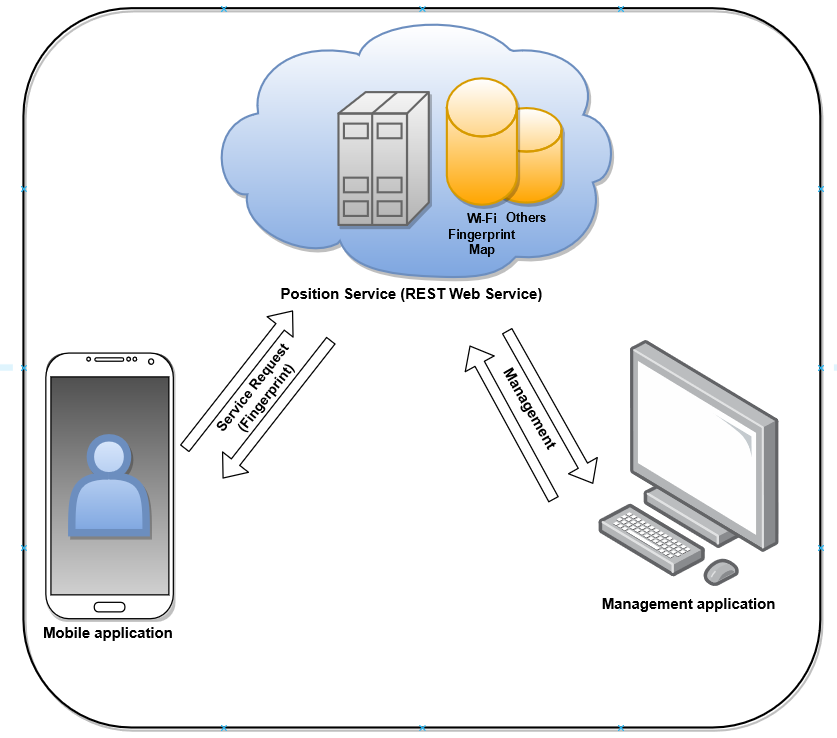
\includegraphics[width=15cm]{arquitetura.png}
		\centering
		\caption{Arquitetura do sistema}

	\end{figure}



\pagebreak

\section{Componentes da infraestrutura de \textit{software} e aplicações}
\subsection{\textit{WebService}}

O \textit{web service} a desenvolver será o \textit{backbone} do funcionamento do sistema. Será ele o responsável por atender pedidos de clientes, devolver recursos requisitados, alterar e guardar dados, implementar medidas de segurança, controlar acessos, notificar utilizadores e garantir uma boa \textit{performance}.\par
O \textit{web service} será desenvolvido segundo uma arquitetura REST (\textit{Representational State Transfer}), com objetivo de desenvolver um sistema com propriedades de usabilidade, simplicidade e escalabilidade. Com estas propriedades, é possível a implementação de um sistema que maximize a escalabilidade e independência, e minimizando comunicações em rede e atrasos.

\pagebreak

\subsubsection{Tecnologias definidas}
O \textit{web service} será desenvolvido em JavaScript, num ambiente Node.js. Esta decisão foi tomada por este ambiente possuir ferramentas que facilitam o desenvolvimento das  funcionalidades. Por exemplo, o módulo Express.js facilita a identificação dos recursos, bem como programação dos \textit{middlewares} que tratam dos pedidos recebidos.\par
Os pedidos e respostas serão enviados utilizando o protocolo HTTP, que é um excelente suporte da característica HATEOAS (\textit{Hypermedia as the Engine onf Application State} de uma REST API - a comunicação será feita utilizando o corpo das mensagens, códigos de resposta, cabeçalhos dos pedidos...\par Os dados transferidos serão organizados em objetos JSON, permitindo armazenar apenas os dados relevantes a cada pedido, e permitindo que, cada pedido, contém informação suficiente para realizar ações sobre recursos no servidor - isto permite manter uma característica \textit{stateless} do servidor.\par
A tecnologia seleccionada para a construção da base de dados foi MongoDB, alojada na \textit{cloud}. Esta decisão deve-se ao fato de, como os dados são transferidos como objetos JSON, facilita o seu armazenamento na base de dados, dado que o MongoDB também utiliza a estrutura JSON para manter informação. A rapidez na pesquisa da base de dados também permite uma melhor \textit{performance} do servidor.

\pagebreak


\subsubsection{Requisitos não-funcionais}

\paragraph{\textit{Proteção da base de dados}} 
A base de dados será descentralizada, e a informação lá contida será armazenada na \textit{cloud}, de modo a adicionar um certo grau de proteção à referida informação: caso ocorram danos ao servidor, a informação da base de dados não é afetada. 

\paragraph{Disponibilidade}
O servidor deve estar disponível 80\% do tempo, a receber e a responder a pedidos. Os restantes 20\% constituem tempo de manutenção do servidor.\par

\paragraph{Desenvolvimento}
Como referido anteriormente, o servidor será desenvolvido em JavaScript, num ambiente Node.js.\par

\paragraph{Segurança}
As funcionalidades disponibilizadas pelo servidor apenas podem ser acedidas por utilizadores com o devido nível de privilégio. Cada utilizador deve-se autenticar antes de utilizar o serviço, e, após autenticação com sucesso, poderá usufruir das funções. \par
Com a  decisão de remover a necessidade de autenticação para os utlizadores \textit{basic}, existe o perigo de ataque por \textit{denial of service}. Para isso o grupo chegou à conclusão que uma solução adequada é limitar o número de pedidos simultâneos que o servidor atende. Ainda não foi decidido um valor concreto para o número de pedidos, devido a ser algo que se obtém através de experimentação e simulação, mas estará presente na implementação final. 

\paragraph{Tempo de resposta}
O servidor não deve demorar mais que dez segundos a atender pedidos recebidos.

\pagebreak

\subsubsection{Funcionalidades do \textit{webservice}}

\paragraph{Localização}
É a funcionalidade principal do \textit{webservice}. O pedido de localização do utilizador deve conter a informção da WiFi \textit{fingerprint} registada pela aplicação móvel (endereços MAC de \textit{access points} próximos, e intensidades medidas), e o \textit{webservice}, após consulta da base de dados, responde com o nome do local onde o utilizador se encontra, ID do ponto de referência mais próximo, nome do ficheiro onde está representada a planta do local (para posteriormente ser apresentado na aplicação móvel) e coordenadas X e Y do ponto de referência para ser apresentado na aplicação.\par
Esta função está disponível para todo o tipo de utilizadores, sejam utilizadores anónimos não registados (\textit{basic}), ou utilizadores registados (\textit{premium}, donos de espaços).

\paragraph{Correção de localização}
Funcionalidade característica de um utilizador \textit{premium}. Um utilizador \textit{premium} que verifique que a informação enviada pelo \textit{webservice} não está de acordo com o local onde se encontra, pode enviar informação a corrigir a resposta do servidor. Este \textit{feedback} será utilizado para melhorar a caracterização do local. Um pedido de correção deve conter dados sobre: ID do utilizador \textit{premium}, etiqueta temporal da correção, ponto de referência fornecido pelo utilizador (que o utilizador considera errado), e o ponto de referência que o utilizador indicou como correto.

\paragraph{Registar um utilizador}
O \textit{webservice} suportará a funcionalidade de adicionar utilizadores. Esta funcionalidade pode ser utilizada por qualquer utilizador (quem desejar pode-se registar, ou um administrador pode ele próprio registar outro utilizador). Utilizadores que se registem podem-se identificar como utilizador \textit{premium} ou dono de espaço.\par

\paragraph{Listar utilizadores}
A funcionalidade de listar os utilizadores atualmente registados será suportada pelo \textit{webservice}. Esta funcionalidade está apenas disponível para administradores. Esta consulta geral fornecerá \textit{username}, ID, nível de privilégio e data de registo de cada utilizador.\par

\paragraph{Consultar utilizador}
É possível pedir ao \textit{webservice} informação sobre um utilizador em específico. Apenas administradores podem solicitar estes dados. Toda a informação presente na base de dados sobre o utilizador é apresentada, nomeadamente dados pessoais (todos os utilizadores), correções feitas (utilizadores \textit{premium}) e espaços atribuídos (donos).\par

\paragraph{Remover utilizador}
Os administradores têm a opção de apagar utilizadores, removendo toda a informação deles da base de dados.\par

\paragraph{Alterar utilizador}
O \textit{webservice} suporta a alteração de dados de utilizadores. Administradores podem alterar qualquer utilizador. Os restantes utilizadores apenas podem alterar informação relativamente a eles próprios.\par

\paragraph{\textit{Login}}
Esta funcionalidade permite aos utilizadores autenticarem-se no \textit{webservice}. Quando a autenticação é feita com sucesso, ou seja, \textit{username} e \textit{password} correspondem à informação na base de dados, o utilizador recebe uma credencial que o identifica, e também o nível de privilégio que ele possui. Esta credencial deve ser enviada juntamente com todos os pedidos, de modo a que o \textit{webservice} possa verificar se o autor do pedido tem permissão para aceder ao recurso requisitado.\par

\paragraph{Listar espaços}
Administradores podem pedir ao servidor uma listagem de todos os locais registados. Juntamente com a identificação dos locais, também segue informação sobre data de adição, nome do ficheiro que contém a planta do local, identidade do dono...\par

\paragraph{Adicionar espaços}
Utilizadores que sejam donos de espaços, e também administradores, podem adicionar novos espaços. Devem fornecer informação da localização geográfica do local, pelo menos três \textit{access points} a partir dos quais se possa identificar o local (especificando informação sobre o endereço MAC de cada um deles, e a respetiva intensidade de sinal), ficheiro da imagem com a representação do local, e outros parâmetros de identificação do local.\par

\paragraph{Listar informação de espaço específico}
Donos de espaços podem alterar a informação apenas dos espaços que lhes pertençam. Administradores podem alterar informação de qualquer espaço.\par

\paragraph{Remover local}
Donos de espaços podem remover os espaços que lhes pertençam. Administradores podem remover qualquer espaço.\par

\paragraph{Alterar informações de espaços}
Donos de espaços podem alterar informação dos espaços que lhes pertençam. Administradores podem alterar informação de qualquer espaço.\par

Estas funcionalidades estão disponíveis através de pedidos HTTP nos URLs disponibilizados e representados na figura abaixo. Toda a informação trocada entre servidor e aplicações estará na forma de objeto JSON, e a segurança está assegurada através da utilização de \textit{tokens} JSON encriptados, que contêm a informação do nível de privilégio do utilizador, e uma duração de validade de uma hora no máximo.

\begin{figure}[!htbp]
		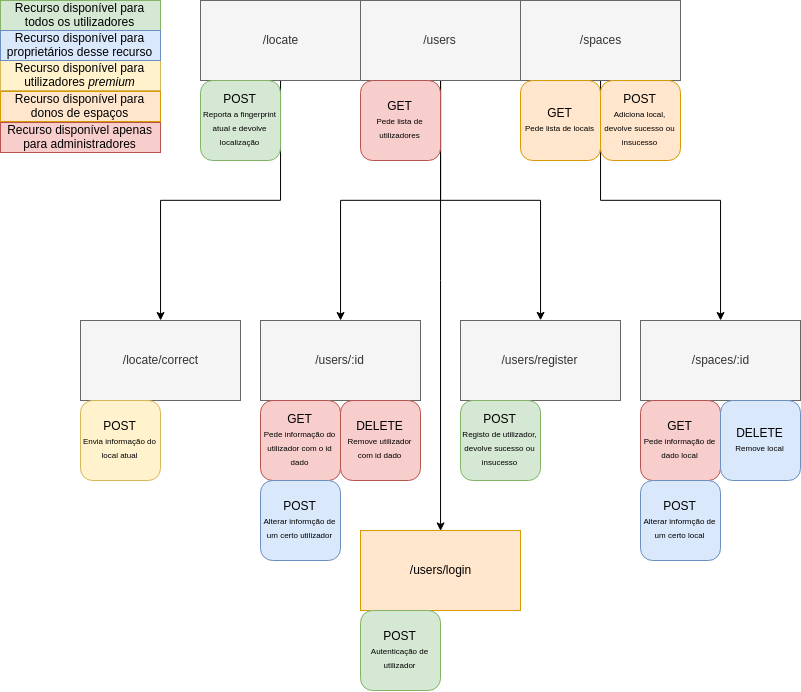
\includegraphics[width=17cm]{webservicestructurev3.png}
		\centering
		\caption{Estrutura de URLs}

	\end{figure}

\pagebreak

\subsection{Aplicação de posicionamento}
A aplicação foi desenvolvida para suportar funcionalidades para todos os tipos de atores deste projeto. Desde a funcionalidade de obter a própria localização, bem como, ferramentas de suporte ao mapeamento e \textit{bootstraping}.

\subsubsection{Estruturação da aplicação}
Ao iniciar a aplicação, o ecrã inicial que irá aparecer será o ecrã de login. Nesse momento será possível iniciar sessão ou escolher entrar em modo anónimo, isto é, entrar como utilizador \textit{basic} que não requer sessão. Caso seja iniciada uma sessão e dependendo do estatuto do utilizador, será redirecionado para um novo ecrã,\textit{Premium} ou dono de espaço.\par

\begin{figure}[!htbp]
		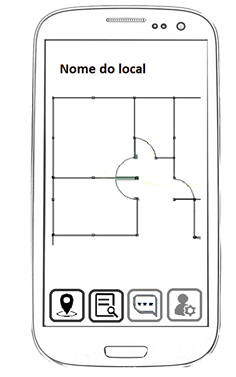
\includegraphics[width=3cm]{app.png}
		\centering
		\caption{Protótipo da aplicação móvel}

	\end{figure}

\subsubsection{Funcionalidades}

\paragraph{Utilizador \textit{basic}}
Um utilizador com estatuto basic tem apenas acesso à funcionalidade de localização do próprio e os seus detalhes, não sendo necessário para esse efeito iniciar sessão com uma conta previamente criada. Isto é, a funcionalidade está disponível a qualquer pessoa que descarregue a aplicação.\par

\paragraph{Utilizador \textit{premium}}
No caso de utilizadores com estatuto premium, para além da funcionalidade anterior descrita, usufruem também do sistema de feedback. Este sistema baseia-se na habilidade do utilizador poder avaliar positivamente ou negativamente a última localização recebida. Isto permite melhorar continuamente a precisão dos mapas.\par

\paragraph{Donos de Espaço}
Quanto aos utilizadores classificados de "Donos de espaço", em adição a todas ferramentas garantidas aos utilizadores já referidos, são responsáveis pela criação inicial de pontos de referência. Este papel requer o preenchimento de detalhes sobre os pontos de referência criados.\par

\pagebreak

\subsubsection{Decisões Android}

\paragraph{\textit{Plug\&Play}}
Um modo que permite qualquer utilizador que descarregue a app a usufruir das funções básicas da aplicação como pedidos de localização e detalhes dos mesmos.\par

\paragraph{\textit{Login}}
Usando as credênciais de uma conta previamente criada com recurso à aplicação web deste mesmo projeto, é possível aceder a funcionalidades reservadas a utilizadores registados.\par

\paragraph{\textit{Cache}}
Com vista a melhorar a resposta aos pedidos de utilizador, a aplicação terá uma funcionalidade de \textit{cache}. Guardar as imagens de mapas recentemente utilizados numa pasta dentro da aplicação, permite reduzir a quantidade de vezes que será necessário descarregar tais mapas a partir do servidor.


\subsubsection{Requisitos não-funcionais}

\paragraph{Segurança}
Uma utilização básica da aplicação não requer qualquer tipo de registo, mas será limitada. Para aceder a mais funcionalidades será necessário iniciar sessão com uma conta previamente criada pela aplicação Web. \par

\paragraph{Portabilidade/Compatibilidade}
Qualquer dispositivo móvel que corra o sistema operativo Android com versão igual ou superior a 4.4.\par

\pagebreak


\subsection{Aplicação gestora de posicionamento}
Como método de gestão de todo o serviço de posicionamento, será desenvolvida uma aplicação de gestão, à qual somente os gestores responsáveis pelo serviço têm permissão de a utilizar. A aplicação permite com que se faça um controlo sobre as bases de dados vinculadas ao servidor \textit{web} à qual esta aplicação estará conectada, nomeadamente, preenchimento de tabelas, alterações nos dados e remoção de dados.\par

\subsubsection{Administradores}
Relativamente ao comportamento dos gestores, cada um deve-se autenticar, de forma a entrar na aplicação. Após sucesso na autenticação, estão disponíveis diversas funcionalidades que se adequam à gestão de todo o serviço de posicionamento. A interface será de tal forma simples e de fácil usabilidade de modo a que, vista de uma perspetiva real, um novo gestor encarregue pela gestão, tenha uma aprendizagem rápida.\par

\begin{figure}[!htbp]
		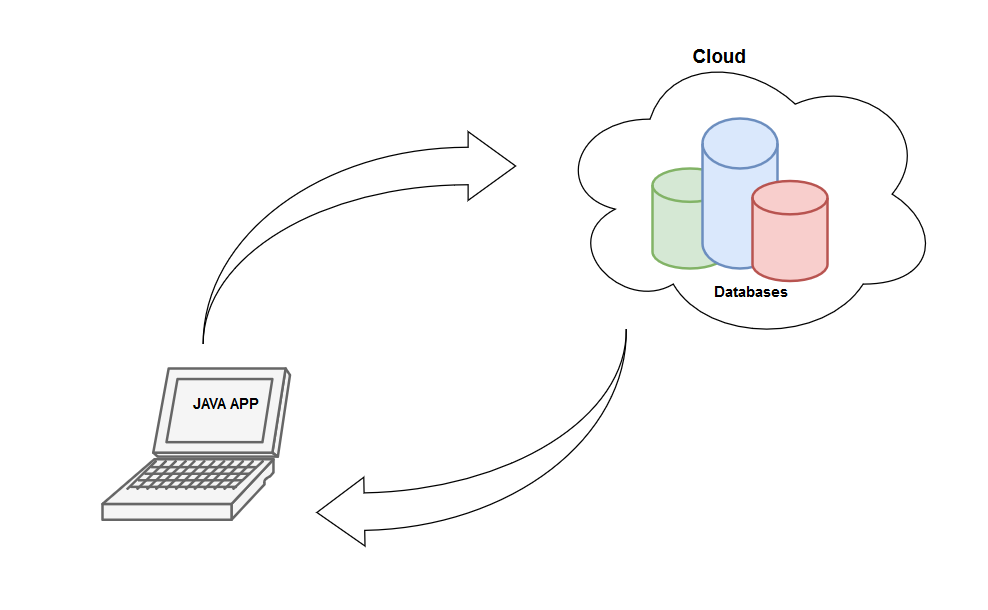
\includegraphics[width=12cm]{sistema.png}
		\centering
		\caption{Comunicação entre aplicação gestora e o servidor}

\end{figure}

\pagebreak

\subsubsection{Funcionalidades}

\paragraph{Adicionar/Alterar/Remover utilizador}
O utilizador remete-se aos clientes que aderiram à aplicação móvel como utilizador premium ou então como dono de espaços;\par

\paragraph{Adicionar/Alterar/Remover local}
É permitido ao gestor de gerir os dados remetentes aos donos de espaços, ou seja, pode adicionar um novo local à base de dados (simbólico) associado a um dono. Porém só poderá fornecer dados gerais à base de dados sobre o local como descrição ou identificador do dono associado. A informação sobre os APs associados ao local deve ser adicionada à base de dados a partir da aplicação de mapeamento;\par

\paragraph{Consulta}
Outras funcionalidades também foram definidas com o propósito de permitir aos gestores de visualizarem o conteúdo atual das bases de dados. Pode consultar dados de um utilizador e caso seja dono de espaço, também pode analisar os locais associados a esse dono.\par

\begin{figure}[!htbp]
		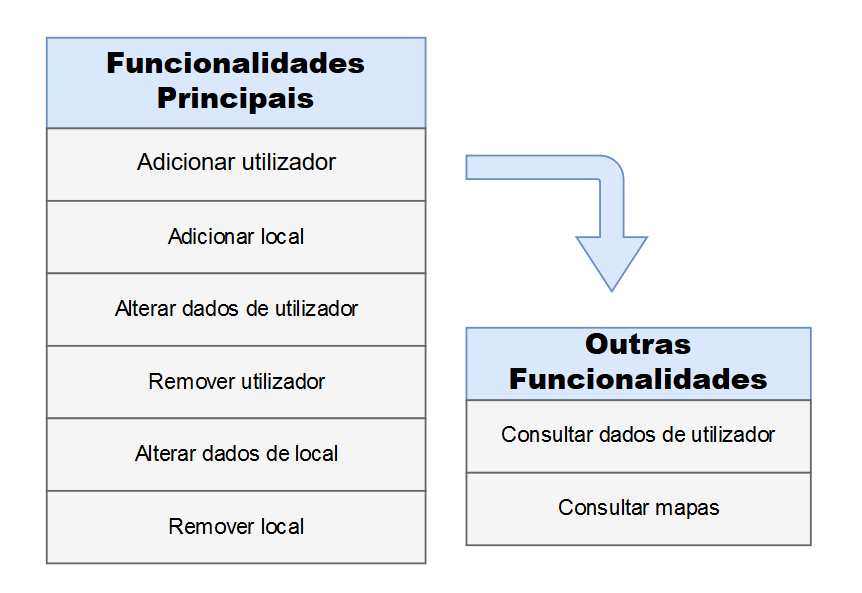
\includegraphics[width=12cm]{Funcionalidades.png}
		\centering
		\caption{Esquema de funcionalidades a serem implementadas}

\end{figure}

\pagebreak

\subsubsection{Requisitos não funcionais}


\paragraph{Requisitos de segurança}
Ao pensar numa situação real em que numa empresa ou organização que está responsável pelo sistema de posicionamento, onde existem vários funcionários no espaço, é necessário que haja uma segurança no acesso à aplicação, em que apenas empregados competentes têm permissão a essas funções. Daí que a aplicação de gestão conterá um nível de acesso à qual somente os gestores têm acesso. Estes devem introduzir seus dados ou \textit{password} (a definir).

\paragraph{Requisitos de usabilidade}
Novos gestores terão uma aprendizagem fácil pois a aplicação de gestão será simples e com recursos de ajuda.


\pagebreak

\section{Modelos de dados}
Os dados estão estruturados representando três entidades distintas: dados de utilizadores, dados de locais e dados de correções de localização feitas por utilizadores \textit{premium}.\par

\subsection{Dados de utilizadores}
A informação armazenada sobre utilizadores tem como objetivo identificar os utilizadores. Os dados armazenados serão os seguintes:

\begin{itemize}[noitemsep]
\item ID do utilizador (identificador único)
\item \textit{E-mail}
\item Nível de privilégio
\item Nome
\item Cartão de crédito (encriptado)
\item CVV (encriptado)
\item Validade do cartão
\item Data de registo
\end{itemize}

\pagebreak

\begin{figure}[!htbp]
  \centering
    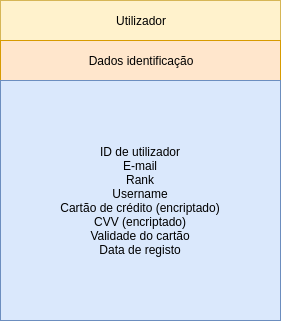
\includegraphics[width=5cm]{modelodadosutilizador.png}
  \caption{Informação relativa a um utilizador}
\end{figure}

Com estes dados é possível suportar funções como, por exemplo, atribuir uma credencial de autenticação correspondente ao nível de privilégio do utilizador, identficar correções feitas caso seja utilizador \textit{premium}...

\pagebreak

\subsection{Dados de locais}
A informação referente aos locais é dividida em dois tipos de informação: dados de identificação e dados de \textit{fingerprinting}. Relativamente aos dados de informação, serão armazenados os seguintes:

\begin{itemize}[noitemsep]
\item ID do local (identificador único)
\item Nome do local
\item Descrição do local
\item Data de adição
\item ID do dono
\item Ficheiro de imagem
\item Número de pontos de referência
\end{itemize}

No caso da informação sobre \textit{fingerprinting}, esta será dividida em pontos de referência, cada um deles possuindo um identificador único. Estes pontos de referência correspondem aos locais exatos, identificados por uma coordenada X e uma coordenada Y, onde são medidas as \textit{fingerprints}. Cada ponto de referência contém uma lista dos \textit{access points} que o caracterizam, e cada \textit{access point} é identificado pelo seu endereço MAC, e intensidade do sinal.

\begin{figure}[!htbp]
  \centering
    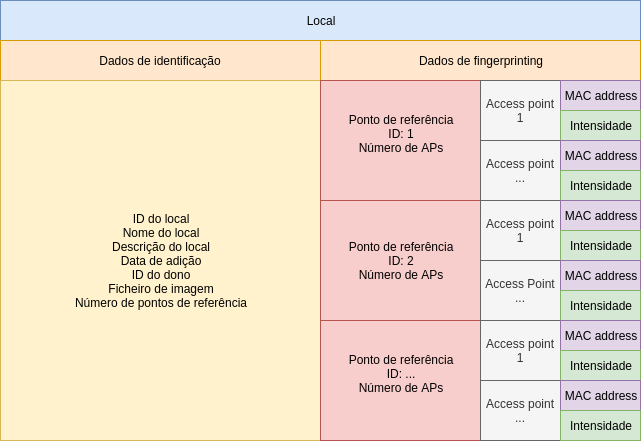
\includegraphics[width=10cm]{modelodadoslocal.png}
  \caption{Informação relativa a um local}
\end{figure}

\pagebreak

\subsection{Dados de correções}
De modo a conseguir utilizar o \textit{feedback} fornecido por utilizadores \textit{premium} de maneira significativa e relevante, as correções por eles efetuadas serão armazenadas separadamente, para facilitar consulta e utilização. A informação armazenada sobre as correções é a seguinte:

\begin{itemize}[noitemsep]
\item Identificador único
\item Quantidade de correções únicas
\item ID do ponto de referência errado
\item ID do ponto de referência indicado pelo utilizador
\end{itemize}

Será ainda guardada informação relativamente a cada correção individual, nomeadamente o ID do utilizador que a efetuou, a data em que ocorreu a correção, e a intensidade de sinal registada.

\begin{figure}[!htbp]
  \centering
    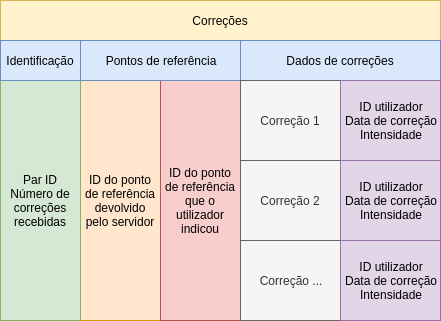
\includegraphics[width=10cm]{modelodadoscorrecoes.png}
  \caption{Informação relativa a correções}
\end{figure}

\pagebreak

\section{Apresentação final}
Para a apresentação final, planeamos mostrar o funcionamento da aplicação em vários aspetos. Primeiro, iremos mostrar a funcionalidade de localização. Supondo que nos localizamos no LAP3 do edifício da Escola de Engenharia da Universidade do Minho, ao solicitar localização, esperamos receber um dos pontos de referência dessa sala, que entretanto estará presente e caracterizada na base de dados. Também iremos mostrar as funcionalidades de registo e \textit{login} de utilizadores, tanto a partir da aplicação móvel como da aplicação gestora (no caso de adicionar um utilizador), bem como adicionar um local e introduzir pontos de referência nele presente, e consultar a informação presente na base de dados relativamente a esse local. Tentaremos também aceder a recursos utilizando uma conta que não tenha acesso a esse recurso, e esperamos obter uma recusa por parte do servidor em atender a esse pedido.\par 
\pagebreak

\section{Conclusão}
Após este planeamento do projeto, podemos afirmar que estamos confiantes na implementação com sucesso deste sistema. Apesar de anteciparmos alguns desafios, nomeadamente na adaptação a novas arquiteturas de \textit{software} e linguagens de programação, temos confiança na nossa capacidade de superarmos essas adversidades e conseguir concluir com sucesso a implementação, atendendo aos requisitos propostos.\par
O planeamento parece-nos robusto, e capaz de orientar bem o desenvolvimento, apesar de certas arestas ainda necessitarem de ser limadas, nomeadamente que informação, especificamente, constará em cada pedido e em cada resposta e quantidade concreta de pedidos simultâneos o servidor atenderá.\par
Com os meios de aprendizagem à nossa disposição, empenho e vontade de entregar uma solução final com qualidade, conseguiremos superar este desafio.\par

\pagebreak








\end{document}




